% Part: sets-functions-relations
% Chapter: infinite
% Section: hilberts-hotel
%
\documentclass[../../../include/open-logic-section]{subfiles}

\begin{document}

\olfileid[fa-IR]{sfr}{infinite}{hilbert}
\olsection{هتل هیلبرت}

مجموعهٔ اعداد طبیعی آشکارا نامتناهی است. بنابراین، اگر نخواهیم اعداد طبیعی
را \emph{مفروض بگیریم}، نخستین گام ما باید توصیف مجموعهٔ نامتناهی با
عبارت‌هایی باشد که نیازی به ذکر خودِ اعداد طبیعی ندارند. اینک رویکردی
دل‌انگیز که هیلبرت در سخنرانی‌ای در سال 1924 عرضه کرد. او از ما می‌خواهد
تصور کنیم
\begin{quote}
[\ldots] هتلی با تعداد متناهی اتاق. هر یک از این اتاق‌ها باید دقیقاً با
یک مهمان اشغال شده باشد. اگر مهمانان اکنون به نحوی اتاق‌هایشان را با هم
عوض کنند، [اما] به‌گونه‌ای که هر اتاق همچنان بیش از یک نفر را در خود جای
ندهد، آنگاه هیچ اتاقی آزاد نخواهد شد و صاحب هتل نمی‌تواند بدین شیوه جایی
تازه برای مهمانی که تازه از راه می‌رسد ایجاد کند [\ldots
\textparagraph \ldots]

اکنون مقرر می‌کنیم که هتل بی‌نهایت اتاقِ شماره‌دارِ $1$، $2$، $3$، $4$،
$5$، \dots داشته باشد و هر یک دقیقاً با یک مهمان اشغال شده باشد. همین که
مهمانی تازه از راه برسد، صاحب هتل فقط باید هر یک از مهمانان قدیمی را به
اتاقی منتقل کند که شماره‌اش یک واحد بیشتر است؛ آنگاه اتاق~$1$ برای مهمان
تازه‌وارد آزاد خواهد شد.
	\begin{center}
		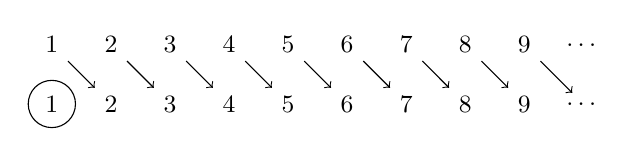
\begin{tikzpicture}[scale = .75]
		\foreach \x in {1, 2, 3, 4, 5, 6, 7, 8, 9}
		{
			\node (\x a) at (\x, 1) {\small{\x}};
			\node (\x b) at (\x, 2) {\small{\x}};
		}
		\node (dotsa) at (10, 1) {\small{\ldots}};
		\node (dotsb) at (10, 2) {\small{\ldots}};
		\draw[->] (1b)--(2a);
		\draw[->] (2b)--(3a);
		\draw[->] (3b)--(4a);
		\draw[->] (4b)--(5a);
		\draw[->] (5b)--(6a);
		\draw[->] (6b)--(7a);
		\draw[->] (7b)--(8a);
		\draw[->] (8b)--(9a);
		\draw[->] (9b)--(dotsa);
		\draw (1,1) circle (.4);
		\end{tikzpicture}
	\end{center}
	(منتشرشده در \citealt[730]{EwaldSieg2013}؛ ترجمهٔ ما)
\end{quote}
نکتهٔ اساسی این است که هتل هیلبرت بی‌نهایت اتاق دارد؛ و می‌توانیم توضیح
او را تعریفی برای معنای این گفته بدانیم. در واقع، رویکرد ددکیند نیز همین
بود (که البته اینجا با زمان‌پریشیِ شدیدی عرضه می‌شود؛ تعریف ددکیند از
\citeyear{Dedekind1888} است):

\begin{defn}\ollabel{defn:DedekindInfinite}
مجموعهٔ $A$ \emph{نامتناهیِ ددکیندی} است اگر و تنها اگر !!a{injection}ای
از~$A$ به یک زیرمجموعهٔ حقیقی از~$A$ وجود داشته باشد. یعنی $o \in A$ای
و !!a{injection}ای چون $f \colon A \to A$ وجود دارند چنان‌که
$o \notin \ran{f}$.
\end{defn}

\end{document}
